\documentclass{article}
\usepackage{tikz}
\usetikzlibrary{spy} 
%\usetikzlibrary{decoration} 
\usepackage{pgf,tikz}
\usepackage{pgfplots,comment}
\usetikzlibrary{spy}
\usetikzlibrary{backgrounds}
\usetikzlibrary{decorations}
\date{}
\begin{document}

\pagestyle{empty}

\pgfdeclarelayer{background layer}
\pgfsetlayers{background layer,main}
\definecolor{darkgray}{rgb}{0.25,0.25,0.25}
\definecolor{lightgray}{rgb}{0.75,0.75,0.75}
%
\begin{figure}[h!]

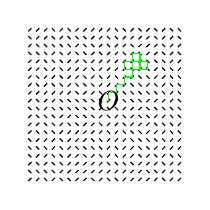
\begin{tikzpicture}
    [scale=0.1,only marks,reddot/.style={fill=red,circle,inner sep=1pt, minimum width=0.5pt},bluedot/.style={fill=blue,circle, inner sep=2pt, minimum width=0.5pt},
    blackdot/.style={fill=black,circle, inner sep=2pt, minimum width=0.5pt},
    yellowdot/.style={fill=yellow,circle, inner sep=2pt, minimum width=0.5pt},
    greendot/.style={fill=green,circle, inner sep=2pt, minimum width=0.5pt},    
     %using the 'spy' to magnify a part of the picture
     spy using outlines={rectangle,lens={scale=3}, size=6cm, connect spies},
     %using the decoration 'brace' (=a curly brace as path replacement)
     %decoration={brace,amplitude=2pt}
]

\draw[color=black] (-9.8,-9.8) -- (-10.2,-10.2);
\draw[color=black] (-10.2,-8.8) -- (-9.8,-9.2);
\draw[color=black] (-9.8,-7.8) -- (-10.2,-8.2);
\draw[color=black] (-10.2,-6.8) -- (-9.8,-7.2);
\draw[color=black] (-10.2,-5.8) -- (-9.8,-6.2);
\draw[color=black] (-10.2,-4.8) -- (-9.8,-5.2);
\draw[color=black] (-9.8,-3.8) -- (-10.2,-4.2);
\draw[color=black] (-9.8,-2.8) -- (-10.2,-3.2);
\draw[color=black] (-9.8,-1.8) -- (-10.2,-2.2);
\draw[color=black] (-10.2,-0.8) -- (-9.8,-1.2);
\draw[color=black] (-9.8,0.2) -- (-10.2,-0.2);
\draw[color=black] (-9.8,1.2) -- (-10.2,0.8);
\draw[color=black] (-9.8,2.2) -- (-10.2,1.8);
\draw[color=black] (-9.8,3.2) -- (-10.2,2.8);
\draw[color=black] (-9.8,4.2) -- (-10.2,3.8);
\draw[color=black] (-9.8,5.2) -- (-10.2,4.8);
\draw[color=black] (-10.2,6.2) -- (-9.8,5.8);
\draw[color=black] (-9.8,7.2) -- (-10.2,6.8);
\draw[color=black] (-10.2,8.2) -- (-9.8,7.8);
\draw[color=black] (-9.8,9.2) -- (-10.2,8.8);
\draw[color=black] (-8.8,-9.8) -- (-9.2,-10.2);
\draw[color=black] (-9.2,-8.8) -- (-8.8,-9.2);
\draw[color=black] (-9.2,-7.8) -- (-8.8,-8.2);
\draw[color=black] (-8.8,-6.8) -- (-9.2,-7.2);
\draw[color=black] (-9.2,-5.8) -- (-8.8,-6.2);
\draw[color=black] (-8.8,-4.8) -- (-9.2,-5.2);
\draw[color=black] (-9.2,-3.8) -- (-8.8,-4.2);
\draw[color=black] (-8.8,-2.8) -- (-9.2,-3.2);
\draw[color=black] (-9.2,-1.8) -- (-8.8,-2.2);
\draw[color=black] (-9.2,-0.8) -- (-8.8,-1.2);
\draw[color=black] (-9.2,0.2) -- (-8.8,-0.2);
\draw[color=black] (-8.8,1.2) -- (-9.2,0.8);
\draw[color=black] (-9.2,2.2) -- (-8.8,1.8);
\draw[color=black] (-9.2,3.2) -- (-8.8,2.8);
\draw[color=black] (-8.8,4.2) -- (-9.2,3.8);
\draw[color=black] (-8.8,5.2) -- (-9.2,4.8);
\draw[color=black] (-9.2,6.2) -- (-8.8,5.8);
\draw[color=black] (-9.2,7.2) -- (-8.8,6.8);
\draw[color=black] (-8.8,8.2) -- (-9.2,7.8);
\draw[color=black] (-8.8,9.2) -- (-9.2,8.8);
\draw[color=black] (-8.2,-9.8) -- (-7.8,-10.2);
\draw[color=black] (-8.2,-8.8) -- (-7.8,-9.2);
\draw[color=black] (-7.8,-7.8) -- (-8.2,-8.2);
\draw[color=black] (-7.8,-6.8) -- (-8.2,-7.2);
\draw[color=black] (-8.2,-5.8) -- (-7.8,-6.2);
\draw[color=black] (-7.8,-4.8) -- (-8.2,-5.2);
\draw[color=black] (-8.2,-3.8) -- (-7.8,-4.2);
\draw[color=black] (-8.2,-2.8) -- (-7.8,-3.2);
\draw[color=black] (-8.2,-1.8) -- (-7.8,-2.2);
\draw[color=black] (-7.8,-0.8) -- (-8.2,-1.2);
\draw[color=black] (-7.8,0.2) -- (-8.2,-0.2);
\draw[color=black] (-7.8,1.2) -- (-8.2,0.8);
\draw[color=black] (-7.8,2.2) -- (-8.2,1.8);
\draw[color=black] (-7.8,3.2) -- (-8.2,2.8);
\draw[color=black] (-8.2,4.2) -- (-7.8,3.8);
\draw[color=black] (-8.2,5.2) -- (-7.8,4.8);
\draw[color=black] (-8.2,6.2) -- (-7.8,5.8);
\draw[color=black] (-8.2,7.2) -- (-7.8,6.8);
\draw[color=black] (-7.8,8.2) -- (-8.2,7.8);
\draw[color=black] (-7.8,9.2) -- (-8.2,8.8);
\draw[color=black] (-6.8,-9.8) -- (-7.2,-10.2);
\draw[color=black] (-7.2,-8.8) -- (-6.8,-9.2);
\draw[color=black] (-7.2,-7.8) -- (-6.8,-8.2);
\draw[color=black] (-7.2,-6.8) -- (-6.8,-7.2);
\draw[color=black] (-6.8,-5.8) -- (-7.2,-6.2);
\draw[color=black] (-6.8,-4.8) -- (-7.2,-5.2);
\draw[color=black] (-7.2,-3.8) -- (-6.8,-4.2);
\draw[color=black] (-7.2,-2.8) -- (-6.8,-3.2);
\draw[color=black] (-7.2,-1.8) -- (-6.8,-2.2);
\draw[color=black] (-7.2,-0.8) -- (-6.8,-1.2);
\draw[color=black] (-6.8,0.2) -- (-7.2,-0.2);
\draw[color=black] (-6.8,1.2) -- (-7.2,0.8);
\draw[color=black] (-7.2,2.2) -- (-6.8,1.8);
\draw[color=black] (-6.8,3.2) -- (-7.2,2.8);
\draw[color=black] (-6.8,4.2) -- (-7.2,3.8);
\draw[color=black] (-7.2,5.2) -- (-6.8,4.8);
\draw[color=black] (-6.8,6.2) -- (-7.2,5.8);
\draw[color=black] (-7.2,7.2) -- (-6.8,6.8);
\draw[color=black] (-7.2,8.2) -- (-6.8,7.8);
\draw[color=black] (-7.2,9.2) -- (-6.8,8.8);
\draw[color=black] (-6.2,-9.8) -- (-5.8,-10.2);
\draw[color=black] (-5.8,-8.8) -- (-6.2,-9.2);
\draw[color=black] (-6.2,-7.8) -- (-5.8,-8.2);
\draw[color=black] (-6.2,-6.8) -- (-5.8,-7.2);
\draw[color=black] (-6.2,-5.8) -- (-5.8,-6.2);
\draw[color=black] (-6.2,-4.8) -- (-5.8,-5.2);
\draw[color=black] (-5.8,-3.8) -- (-6.2,-4.2);
\draw[color=black] (-5.8,-2.8) -- (-6.2,-3.2);
\draw[color=black] (-5.8,-1.8) -- (-6.2,-2.2);
\draw[color=black] (-6.2,-0.8) -- (-5.8,-1.2);
\draw[color=black] (-6.2,0.2) -- (-5.8,-0.2);
\draw[color=black] (-5.8,1.2) -- (-6.2,0.8);
\draw[color=black] (-6.2,2.2) -- (-5.8,1.8);
\draw[color=black] (-6.2,3.2) -- (-5.8,2.8);
\draw[color=black] (-6.2,4.2) -- (-5.8,3.8);
\draw[color=black] (-6.2,5.2) -- (-5.8,4.8);
\draw[color=black] (-6.2,6.2) -- (-5.8,5.8);
\draw[color=black] (-6.2,7.2) -- (-5.8,6.8);
\draw[color=black] (-5.8,8.2) -- (-6.2,7.8);
\draw[color=black] (-5.8,9.2) -- (-6.2,8.8);
\draw[color=black] (-5.2,-9.8) -- (-4.8,-10.2);
\draw[color=black] (-4.8,-8.8) -- (-5.2,-9.2);
\draw[color=black] (-4.8,-7.8) -- (-5.2,-8.2);
\draw[color=black] (-4.8,-6.8) -- (-5.2,-7.2);
\draw[color=black] (-4.8,-5.8) -- (-5.2,-6.2);
\draw[color=black] (-4.8,-4.8) -- (-5.2,-5.2);
\draw[color=black] (-4.8,-3.8) -- (-5.2,-4.2);
\draw[color=black] (-5.2,-2.8) -- (-4.8,-3.2);
\draw[color=black] (-4.8,-1.8) -- (-5.2,-2.2);
\draw[color=black] (-5.2,-0.8) -- (-4.8,-1.2);
\draw[color=black] (-5.2,0.2) -- (-4.8,-0.2);
\draw[color=black] (-4.8,1.2) -- (-5.2,0.8);
\draw[color=black] (-4.8,2.2) -- (-5.2,1.8);
\draw[color=black] (-4.8,3.2) -- (-5.2,2.8);
\draw[color=black] (-4.8,4.2) -- (-5.2,3.8);
\draw[color=black] (-4.8,5.2) -- (-5.2,4.8);
\draw[color=black] (-4.8,6.2) -- (-5.2,5.8);
\draw[color=black] (-5.2,7.2) -- (-4.8,6.8);
\draw[color=black] (-5.2,8.2) -- (-4.8,7.8);
\draw[color=black] (-5.2,9.2) -- (-4.8,8.8);
\draw[color=black] (-3.8,-9.8) -- (-4.2,-10.2);
\draw[color=black] (-3.8,-8.8) -- (-4.2,-9.2);
\draw[color=black] (-3.8,-7.8) -- (-4.2,-8.2);
\draw[color=black] (-3.8,-6.8) -- (-4.2,-7.2);
\draw[color=black] (-4.2,-5.8) -- (-3.8,-6.2);
\draw[color=black] (-3.8,-4.8) -- (-4.2,-5.2);
\draw[color=black] (-3.8,-3.8) -- (-4.2,-4.2);
\draw[color=black] (-4.2,-2.8) -- (-3.8,-3.2);
\draw[color=black] (-4.2,-1.8) -- (-3.8,-2.2);
\draw[color=black] (-4.2,-0.8) -- (-3.8,-1.2);
\draw[color=black] (-4.2,0.2) -- (-3.8,-0.2);
\draw[color=black] (-4.2,1.2) -- (-3.8,0.8);
\draw[color=black] (-4.2,2.2) -- (-3.8,1.8);
\draw[color=black] (-3.8,3.2) -- (-4.2,2.8);
\draw[color=black] (-3.8,4.2) -- (-4.2,3.8);
\draw[color=black] (-3.8,5.2) -- (-4.2,4.8);
\draw[color=black] (-4.2,6.2) -- (-3.8,5.8);
\draw[color=black] (-3.8,7.2) -- (-4.2,6.8);
\draw[color=black] (-4.2,8.2) -- (-3.8,7.8);
\draw[color=black] (-3.8,9.2) -- (-4.2,8.8);
\draw[color=black] (-2.8,-9.8) -- (-3.2,-10.2);
\draw[color=black] (-2.8,-8.8) -- (-3.2,-9.2);
\draw[color=black] (-2.8,-7.8) -- (-3.2,-8.2);
\draw[color=black] (-3.2,-6.8) -- (-2.8,-7.2);
\draw[color=black] (-3.2,-5.8) -- (-2.8,-6.2);
\draw[color=black] (-2.8,-4.8) -- (-3.2,-5.2);
\draw[color=black] (-2.8,-3.8) -- (-3.2,-4.2);
\draw[color=black] (-2.8,-2.8) -- (-3.2,-3.2);
\draw[color=black] (-3.2,-1.8) -- (-2.8,-2.2);
\draw[color=black] (-3.2,-0.8) -- (-2.8,-1.2);
\draw[color=black] (-3.2,0.2) -- (-2.8,-0.2);
\draw[color=black] (-2.8,1.2) -- (-3.2,0.8);
\draw[color=black] (-3.2,2.2) -- (-2.8,1.8);
\draw[color=black] (-3.2,3.2) -- (-2.8,2.8);
\draw[color=black] (-2.8,4.2) -- (-3.2,3.8);
\draw[color=black] (-3.2,5.2) -- (-2.8,4.8);
\draw[color=black] (-3.2,6.2) -- (-2.8,5.8);
\draw[color=black] (-3.2,7.2) -- (-2.8,6.8);
\draw[color=black] (-3.2,8.2) -- (-2.8,7.8);
\draw[color=black] (-2.8,9.2) -- (-3.2,8.8);
\draw[color=black] (-2.2,-9.8) -- (-1.8,-10.2);
\draw[color=black] (-1.8,-8.8) -- (-2.2,-9.2);
\draw[color=black] (-1.8,-7.8) -- (-2.2,-8.2);
\draw[color=black] (-1.8,-6.8) -- (-2.2,-7.2);
\draw[color=black] (-2.2,-5.8) -- (-1.8,-6.2);
\draw[color=black] (-2.2,-4.8) -- (-1.8,-5.2);
\draw[color=black] (-1.8,-3.8) -- (-2.2,-4.2);
\draw[color=black] (-1.8,-2.8) -- (-2.2,-3.2);
\draw[color=black] (-2.2,-1.8) -- (-1.8,-2.2);
\draw[color=black] (-2.2,-0.8) -- (-1.8,-1.2);
\draw[color=black] (-2.2,0.2) -- (-1.8,-0.2);
\draw[color=black] (-1.8,1.2) -- (-2.2,0.8);
\draw[color=black] (-2.2,2.2) -- (-1.8,1.8);
\draw[color=black] (-1.8,3.2) -- (-2.2,2.8);
\draw[color=black] (-2.2,4.2) -- (-1.8,3.8);
\draw[color=black] (-1.8,5.2) -- (-2.2,4.8);
\draw[color=black] (-1.8,6.2) -- (-2.2,5.8);
\draw[color=black] (-2.2,7.2) -- (-1.8,6.8);
\draw[color=black] (-1.8,8.2) -- (-2.2,7.8);
\draw[color=black] (-1.8,9.2) -- (-2.2,8.8);
\draw[color=black] (-0.8,-9.8) -- (-1.2,-10.2);
\draw[color=black] (-0.8,-8.8) -- (-1.2,-9.2);
\draw[color=black] (-0.8,-7.8) -- (-1.2,-8.2);
\draw[color=black] (-1.2,-6.8) -- (-0.8,-7.2);
\draw[color=black] (-1.2,-5.8) -- (-0.8,-6.2);
\draw[color=black] (-1.2,-4.8) -- (-0.8,-5.2);
\draw[color=black] (-0.8,-3.8) -- (-1.2,-4.2);
\draw[color=black] (-1.2,-2.8) -- (-0.8,-3.2);
\draw[color=black] (-0.8,-1.8) -- (-1.2,-2.2);
\draw[color=black] (-0.8,-0.8) -- (-1.2,-1.2);
\draw[color=black] (-1.2,0.2) -- (-0.8,-0.2);
\draw[color=black] (-1.2,1.2) -- (-0.8,0.8);
\draw[color=black] (-0.8,2.2) -- (-1.2,1.8);
\draw[color=black] (-1.2,3.2) -- (-0.8,2.8);
\draw[color=black] (-0.8,4.2) -- (-1.2,3.8);
\draw[color=black] (-0.8,5.2) -- (-1.2,4.8);
\draw[color=black] (-1.2,6.2) -- (-0.8,5.8);
\draw[color=black] (-0.8,7.2) -- (-1.2,6.8);
\draw[color=black] (-0.8,8.2) -- (-1.2,7.8);
\draw[color=black] (-0.8,9.2) -- (-1.2,8.8);
\draw[color=black] (-0.2,-9.8) -- (0.2,-10.2);
\draw[color=black] (0.2,-8.8) -- (-0.2,-9.2);
\draw[color=black] (-0.2,-7.8) -- (0.2,-8.2);
\draw[color=black] (0.2,-6.8) -- (-0.2,-7.2);
\draw[color=black] (0.2,-5.8) -- (-0.2,-6.2);
\draw[color=black] (0.2,-4.8) -- (-0.2,-5.2);
\draw[color=black] (-0.2,-3.8) -- (0.2,-4.2);
\draw[color=black] (0.2,-2.8) -- (-0.2,-3.2);
\draw[color=black] (-0.2,-1.8) -- (0.2,-2.2);
\draw[color=black] (-0.2,-0.8) -- (0.2,-1.2);
\draw[color=black] (0.2,0.2) -- (-0.2,-0.2);
\draw[color=black] (0.2,1.2) -- (-0.2,0.8);
\draw[color=black] (0.2,2.2) -- (-0.2,1.8);
\draw[color=black] (0.2,3.2) -- (-0.2,2.8);
\draw[color=black] (0.2,4.2) -- (-0.2,3.8);
\draw[color=black] (0.2,5.2) -- (-0.2,4.8);
\draw[color=black] (0.2,6.2) -- (-0.2,5.8);
\draw[color=black] (-0.2,7.2) -- (0.2,6.8);
\draw[color=black] (-0.2,8.2) -- (0.2,7.8);
\draw[color=black] (0.2,9.2) -- (-0.2,8.8);
\draw[color=black] (0.8,-9.8) -- (1.2,-10.2);
\draw[color=black] (1.2,-8.8) -- (0.8,-9.2);
\draw[color=black] (0.8,-7.8) -- (1.2,-8.2);
\draw[color=black] (0.8,-6.8) -- (1.2,-7.2);
\draw[color=black] (0.8,-5.8) -- (1.2,-6.2);
\draw[color=black] (1.2,-4.8) -- (0.8,-5.2);
\draw[color=black] (1.2,-3.8) -- (0.8,-4.2);
\draw[color=black] (1.2,-2.8) -- (0.8,-3.2);
\draw[color=black] (1.2,-1.8) -- (0.8,-2.2);
\draw[color=black] (0.8,-0.8) -- (1.2,-1.2);
\draw[color=black] (1.2,0.2) -- (0.8,-0.2);
\draw[color=black] (1.2,1.2) -- (0.8,0.8);
\draw[color=black] (1.2,2.2) -- (0.8,1.8);
\draw[color=black] (0.8,3.2) -- (1.2,2.8);
\draw[color=black] (1.2,4.2) -- (0.8,3.8);
\draw[color=black] (1.2,5.2) -- (0.8,4.8);
\draw[color=black] (1.2,6.2) -- (0.8,5.8);
\draw[color=black] (1.2,7.2) -- (0.8,6.8);
\draw[color=black] (0.8,8.2) -- (1.2,7.8);
\draw[color=black] (0.8,9.2) -- (1.2,8.8);
\draw[color=black] (2.2,-9.8) -- (1.8,-10.2);
\draw[color=black] (2.2,-8.8) -- (1.8,-9.2);
\draw[color=black] (1.8,-7.8) -- (2.2,-8.2);
\draw[color=black] (2.2,-6.8) -- (1.8,-7.2);
\draw[color=black] (2.2,-5.8) -- (1.8,-6.2);
\draw[color=black] (2.2,-4.8) -- (1.8,-5.2);
\draw[color=black] (1.8,-3.8) -- (2.2,-4.2);
\draw[color=black] (1.8,-2.8) -- (2.2,-3.2);
\draw[color=black] (1.8,-1.8) -- (2.2,-2.2);
\draw[color=black] (2.2,-0.8) -- (1.8,-1.2);
\draw[color=black] (1.8,0.2) -- (2.2,-0.2);
\draw[color=black] (1.8,1.2) -- (2.2,0.8);
\draw[color=black] (2.2,2.2) -- (1.8,1.8);
\draw[color=black] (2.2,3.2) -- (1.8,2.8);
\draw[color=black] (2.2,4.2) -- (1.8,3.8);
\draw[color=black] (2.2,5.2) -- (1.8,4.8);
\draw[color=black] (1.8,6.2) -- (2.2,5.8);
\draw[color=black] (2.2,7.2) -- (1.8,6.8);
\draw[color=black] (2.2,8.2) -- (1.8,7.8);
\draw[color=black] (1.8,9.2) -- (2.2,8.8);
\draw[color=black] (3.2,-9.8) -- (2.8,-10.2);
\draw[color=black] (3.2,-8.8) -- (2.8,-9.2);
\draw[color=black] (2.8,-7.8) -- (3.2,-8.2);
\draw[color=black] (3.2,-6.8) -- (2.8,-7.2);
\draw[color=black] (3.2,-5.8) -- (2.8,-6.2);
\draw[color=black] (2.8,-4.8) -- (3.2,-5.2);
\draw[color=black] (2.8,-3.8) -- (3.2,-4.2);
\draw[color=black] (3.2,-2.8) -- (2.8,-3.2);
\draw[color=black] (3.2,-1.8) -- (2.8,-2.2);
\draw[color=black] (3.2,-0.8) -- (2.8,-1.2);
\draw[color=black] (2.8,0.2) -- (3.2,-0.2);
\draw[color=black] (2.8,1.2) -- (3.2,0.8);
\draw[color=black] (2.8,2.2) -- (3.2,1.8);
\draw[color=black] (3.2,3.2) -- (2.8,2.8);
\draw[color=black] (2.8,4.2) -- (3.2,3.8);
\draw[color=black] (3.2,5.2) -- (2.8,4.8);
\draw[color=black] (3.2,6.2) -- (2.8,5.8);
\draw[color=black] (2.8,7.2) -- (3.2,6.8);
\draw[color=black] (3.2,8.2) -- (2.8,7.8);
\draw[color=black] (3.2,9.2) -- (2.8,8.8);
\draw[color=black] (4.2,-9.8) -- (3.8,-10.2);
\draw[color=black] (4.2,-8.8) -- (3.8,-9.2);
\draw[color=black] (4.2,-7.8) -- (3.8,-8.2);
\draw[color=black] (3.8,-6.8) -- (4.2,-7.2);
\draw[color=black] (3.8,-5.8) -- (4.2,-6.2);
\draw[color=black] (3.8,-4.8) -- (4.2,-5.2);
\draw[color=black] (3.8,-3.8) -- (4.2,-4.2);
\draw[color=black] (4.2,-2.8) -- (3.8,-3.2);
\draw[color=black] (3.8,-1.8) -- (4.2,-2.2);
\draw[color=black] (4.2,-0.8) -- (3.8,-1.2);
\draw[color=black] (3.8,0.2) -- (4.2,-0.2);
\draw[color=black] (3.8,1.2) -- (4.2,0.8);
\draw[color=black] (3.8,2.2) -- (4.2,1.8);
\draw[color=black] (3.8,3.2) -- (4.2,2.8);
\draw[color=black] (4.2,4.2) -- (3.8,3.8);
\draw[color=black] (4.2,5.2) -- (3.8,4.8);
\draw[color=black] (3.8,6.2) -- (4.2,5.8);
\draw[color=black] (4.2,7.2) -- (3.8,6.8);
\draw[color=black] (4.2,8.2) -- (3.8,7.8);
\draw[color=black] (3.8,9.2) -- (4.2,8.8);
\draw[color=black] (5.2,-9.8) -- (4.8,-10.2);
\draw[color=black] (4.8,-8.8) -- (5.2,-9.2);
\draw[color=black] (5.2,-7.8) -- (4.8,-8.2);
\draw[color=black] (5.2,-6.8) -- (4.8,-7.2);
\draw[color=black] (4.8,-5.8) -- (5.2,-6.2);
\draw[color=black] (4.8,-4.8) -- (5.2,-5.2);
\draw[color=black] (5.2,-3.8) -- (4.8,-4.2);
\draw[color=black] (5.2,-2.8) -- (4.8,-3.2);
\draw[color=black] (4.8,-1.8) -- (5.2,-2.2);
\draw[color=black] (4.8,-0.8) -- (5.2,-1.2);
\draw[color=black] (5.2,0.2) -- (4.8,-0.2);
\draw[color=black] (4.8,1.2) -- (5.2,0.8);
\draw[color=black] (5.2,2.2) -- (4.8,1.8);
\draw[color=black] (4.8,3.2) -- (5.2,2.8);
\draw[color=black] (4.8,4.2) -- (5.2,3.8);
\draw[color=black] (4.8,5.2) -- (5.2,4.8);
\draw[color=black] (5.2,6.2) -- (4.8,5.8);
\draw[color=black] (5.2,7.2) -- (4.8,6.8);
\draw[color=black] (5.2,8.2) -- (4.8,7.8);
\draw[color=black] (5.2,9.2) -- (4.8,8.8);
\draw[color=black] (6.2,-9.8) -- (5.8,-10.2);
\draw[color=black] (5.8,-8.8) -- (6.2,-9.2);
\draw[color=black] (6.2,-7.8) -- (5.8,-8.2);
\draw[color=black] (5.8,-6.8) -- (6.2,-7.2);
\draw[color=black] (6.2,-5.8) -- (5.8,-6.2);
\draw[color=black] (5.8,-4.8) -- (6.2,-5.2);
\draw[color=black] (6.2,-3.8) -- (5.8,-4.2);
\draw[color=black] (5.8,-2.8) -- (6.2,-3.2);
\draw[color=black] (6.2,-1.8) -- (5.8,-2.2);
\draw[color=black] (5.8,-0.8) -- (6.2,-1.2);
\draw[color=black] (6.2,0.2) -- (5.8,-0.2);
\draw[color=black] (5.8,1.2) -- (6.2,0.8);
\draw[color=black] (5.8,2.2) -- (6.2,1.8);
\draw[color=black] (6.2,3.2) -- (5.8,2.8);
\draw[color=black] (6.2,4.2) -- (5.8,3.8);
\draw[color=black] (5.8,5.2) -- (6.2,4.8);
\draw[color=black] (6.2,6.2) -- (5.8,5.8);
\draw[color=black] (6.2,7.2) -- (5.8,6.8);
\draw[color=black] (5.8,8.2) -- (6.2,7.8);
\draw[color=black] (5.8,9.2) -- (6.2,8.8);
\draw[color=black] (6.8,-9.8) -- (7.2,-10.2);
\draw[color=black] (7.2,-8.8) -- (6.8,-9.2);
\draw[color=black] (6.8,-7.8) -- (7.2,-8.2);
\draw[color=black] (7.2,-6.8) -- (6.8,-7.2);
\draw[color=black] (7.2,-5.8) -- (6.8,-6.2);
\draw[color=black] (6.8,-4.8) -- (7.2,-5.2);
\draw[color=black] (7.2,-3.8) -- (6.8,-4.2);
\draw[color=black] (6.8,-2.8) -- (7.2,-3.2);
\draw[color=black] (7.2,-1.8) -- (6.8,-2.2);
\draw[color=black] (6.8,-0.8) -- (7.2,-1.2);
\draw[color=black] (7.2,0.2) -- (6.8,-0.2);
\draw[color=black] (6.8,1.2) -- (7.2,0.8);
\draw[color=black] (7.2,2.2) -- (6.8,1.8);
\draw[color=black] (7.2,3.2) -- (6.8,2.8);
\draw[color=black] (6.8,4.2) -- (7.2,3.8);
\draw[color=black] (6.8,5.2) -- (7.2,4.8);
\draw[color=black] (6.8,6.2) -- (7.2,5.8);
\draw[color=black] (6.8,7.2) -- (7.2,6.8);
\draw[color=black] (7.2,8.2) -- (6.8,7.8);
\draw[color=black] (7.2,9.2) -- (6.8,8.8);
\draw[color=black] (8.2,-9.8) -- (7.8,-10.2);
\draw[color=black] (8.2,-8.8) -- (7.8,-9.2);
\draw[color=black] (8.2,-7.8) -- (7.8,-8.2);
\draw[color=black] (7.8,-6.8) -- (8.2,-7.2);
\draw[color=black] (8.2,-5.8) -- (7.8,-6.2);
\draw[color=black] (8.2,-4.8) -- (7.8,-5.2);
\draw[color=black] (7.8,-3.8) -- (8.2,-4.2);
\draw[color=black] (7.8,-2.8) -- (8.2,-3.2);
\draw[color=black] (7.8,-1.8) -- (8.2,-2.2);
\draw[color=black] (7.8,-0.8) -- (8.2,-1.2);
\draw[color=black] (8.2,0.2) -- (7.8,-0.2);
\draw[color=black] (8.2,1.2) -- (7.8,0.8);
\draw[color=black] (7.8,2.2) -- (8.2,1.8);
\draw[color=black] (7.8,3.2) -- (8.2,2.8);
\draw[color=black] (7.8,4.2) -- (8.2,3.8);
\draw[color=black] (8.2,5.2) -- (7.8,4.8);
\draw[color=black] (8.2,6.2) -- (7.8,5.8);
\draw[color=black] (8.2,7.2) -- (7.8,6.8);
\draw[color=black] (8.2,8.2) -- (7.8,7.8);
\draw[color=black] (7.8,9.2) -- (8.2,8.8);
\draw[color=black] (9.2,-9.8) -- (8.8,-10.2);
\draw[color=black] (8.8,-8.8) -- (9.2,-9.2);
\draw[color=black] (9.2,-7.8) -- (8.8,-8.2);
\draw[color=black] (8.8,-6.8) -- (9.2,-7.2);
\draw[color=black] (9.2,-5.8) -- (8.8,-6.2);
\draw[color=black] (9.2,-4.8) -- (8.8,-5.2);
\draw[color=black] (8.8,-3.8) -- (9.2,-4.2);
\draw[color=black] (9.2,-2.8) -- (8.8,-3.2);
\draw[color=black] (8.8,-1.8) -- (9.2,-2.2);
\draw[color=black] (8.8,-0.8) -- (9.2,-1.2);
\draw[color=black] (8.8,0.2) -- (9.2,-0.2);
\draw[color=black] (8.8,1.2) -- (9.2,0.8);
\draw[color=black] (8.8,2.2) -- (9.2,1.8);
\draw[color=black] (8.8,3.2) -- (9.2,2.8);
\draw[color=black] (9.2,4.2) -- (8.8,3.8);
\draw[color=black] (9.2,5.2) -- (8.8,4.8);
\draw[color=black] (8.8,6.2) -- (9.2,5.8);
\draw[color=black] (9.2,7.2) -- (8.8,6.8);
\draw[color=black] (8.8,8.2) -- (9.2,7.8);
\draw[color=black] (8.8,9.2) -- (9.2,8.8);
\draw[color=green] (0,0) -- (0,1);\draw[color=green] (0,1) -- (1,1);\draw[color=green] (1,1) -- (1,2);\draw[color=green] (1,2) -- (2,2);\draw[color=green] (2,2) -- (2,3);\draw[color=green] (2,3) -- (3,3);\draw[color=green] (3,3) -- (3,4);\draw[color=green] (3,4) -- (2,4);\draw[color=green] (2,4) -- (2,5);\draw[color=green] (2,5) -- (3,5);\draw[color=green] (3,5) -- (3,6);\draw[color=green] (3,6) -- (4,6);\draw[color=green] (4,6) -- (4,5);\draw[color=green] (4,5) -- (5,5);\draw[color=green] (5,5) -- (5,4);\draw[color=green] (5,4) -- (4,4);\draw[color=green] (4,4) -- (4,5);\draw[color=green] (4,5) -- (3,5);\draw[color=green] (3,5) -- (3,4);\draw[color=green] (3,4) -- (4,4);
\node at (0,0)[black]{$O$};

\end{tikzpicture}

\end{figure}
\end{document}
